\documentclass{article}
\usepackage[utf8]{inputenc}
\usepackage[latin]{babel}
\usepackage[T1]{fontenc}
\usepackage{graphicx}
\usepackage{hyperref}
\usepackage{float}
\usepackage{glossaries}

\makeglossaries

\graphicspath{ {./image/} }

\usepackage{lmodern,tikz,lipsum}
\newcommand\framethispage[1][2cm]{%
    \tikz[overlay,remember picture,line width=2pt]
    \draw([xshift=(#1),yshift=(-#1)]current page.north west)rectangle
         ([xshift=(-#1),yshift=(#1)]current page.south east);%
}

\usepackage{wrapfig}
\usepackage{threeparttable} 

\usepackage{caption}
\DeclareCaptionFormat{legend}{#3}
\captionsetup{format = legend, font = it}

\usepackage{lipsum}
    
\begin{document}

\newcommand\interline{0.3cm}
\thispagestyle{empty}
%\fbox{
%\begin{minipage}{\textwidth}
\begin{titlepage}
\framethispage[1.9cm]% le cadre est à 2 cm des bords de la feuille
\begin{center}

\vspace{1cm}
\begin{minipage}[b]{3.5cm}

\includegraphics[width=2cm]{LOGO_RVB_grand-UM.jpg}
\end{minipage}\begin{minipage}[b]{3.5cm}


\includegraphics[width=2cm]{lirmm.fr.png}
\end{minipage}\begin{minipage}[b]{3.5cm}


\includegraphics[width=2cm]{logo.png}
\end{minipage}\begin{minipage}[b]{3cm}


\includegraphics[width=2cm]{LOGO_DTP_INFORMATIQUE.jpg}
\end{minipage}
\vspace{1cm}

\Large{Université de Montpellier\\
\vspace{\interline}

Faculté des Sciences} \\
\vspace{2cm}

{\huge MASTER 2 INFORMATIQUE \\
\vspace{\interline}

Parcours IMAGINE \\}
\vspace{2cm}
{\huge \textbf{Automatisation du prétraitement de photos de mandrills}}\\
\vspace{2cm}
Effectué au LIRMM et au CNRS \\
\vspace{\interline}
du 31 janvier au 29 juillet 2022 \\
\vspace{\interline}
par Maxime BOUCHER\\
\vspace{2cm}
Tuteurs en entreprise: William Puech et Julien Renoult \\
\vspace{\interline}
Tuteur à l'université: Madalina Croitoru 
\end{center}
\end{titlepage}


\newglossaryentry{latex}
{
    name=latex,
    description={Is a markup language specially suited 
    for scientific documents}
}

\newglossaryentry{maths}
{
    name=mathematics,
    description={Mathematics is what mathematicians do}
}


\newpage

\newpage

\renewcommand{\contentsname}{Table des matières}
\tableofcontents

\newpage


\renewcommand{\listfigurename}{Table des figures}
\listoffigures

\newpage

\section{Introduction}
The \Gls{latex} typesetting markup language is specially suitable 
for documents that include \gls{maths}. 


\section{Présentation de l'entreprise} 

\section{Présentation de la mission (facultatif, nécessaire si la présentation du sujet dans l'introduction ne suffit pas) }

\section{Environnement technique} 

\section{Veille technologique ou appropriation scientifique (facultatif)} 

\section{Travaux effectués} 

\subsection{Classification des images par qualité, face profils}
L'objectif fixé à la première visio conférence a été déterminé : faire de la classification sur la qualité des photographies des mandrills.\\

J'ai donc commencé par faire du transfer learning avec MobileNet V2, un CNN existant de Google adapté aux mobiles (c'est-à-dire, très rapide et plutôt performant) pour essayer d'adapter un modèle avec les poids ImageNet pour la classification de la qualité des photographies. Notre dataset ressemble aux images ci-dessous, avec FaceQual0-3 en label de qualité, 3 étant la meilleure qualité.

\begin{center}
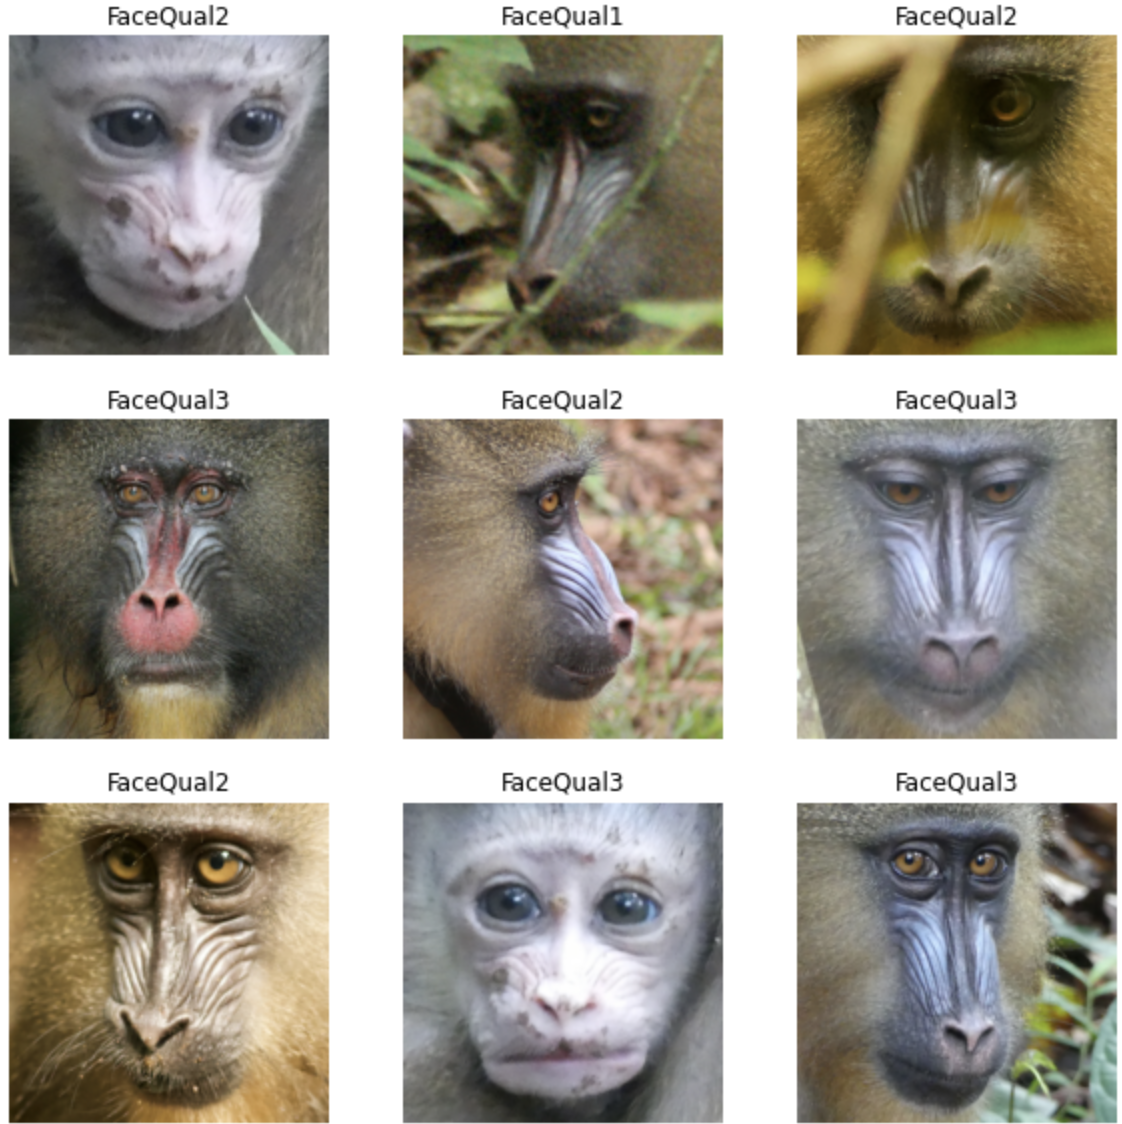
\includegraphics[width=200pt]{imgs/qualité/cr1/dataset.png}
\end{center}

Les premiers résultats semblent bons à première vue : 85\% d'accuracy sur une classification simple.

\begin{center}
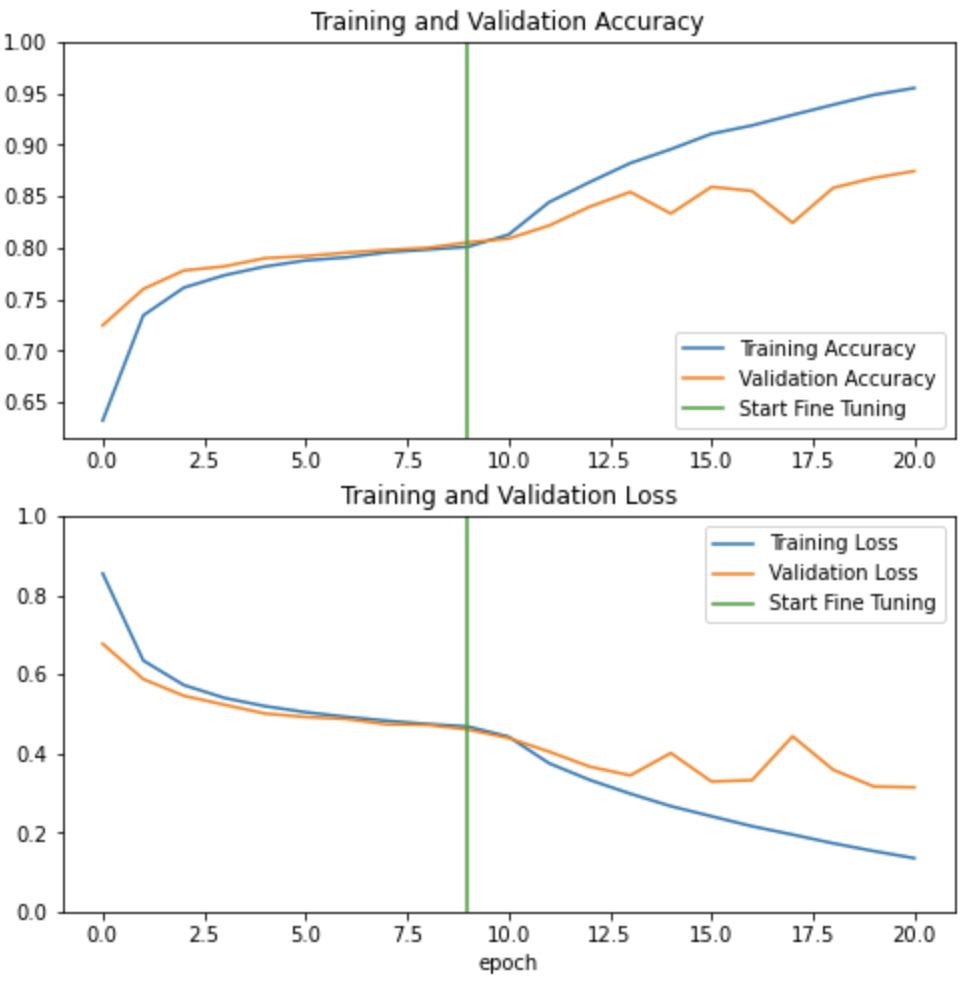
\includegraphics[width=200pt]{imgs/qualité/cr1/resultat1.png}
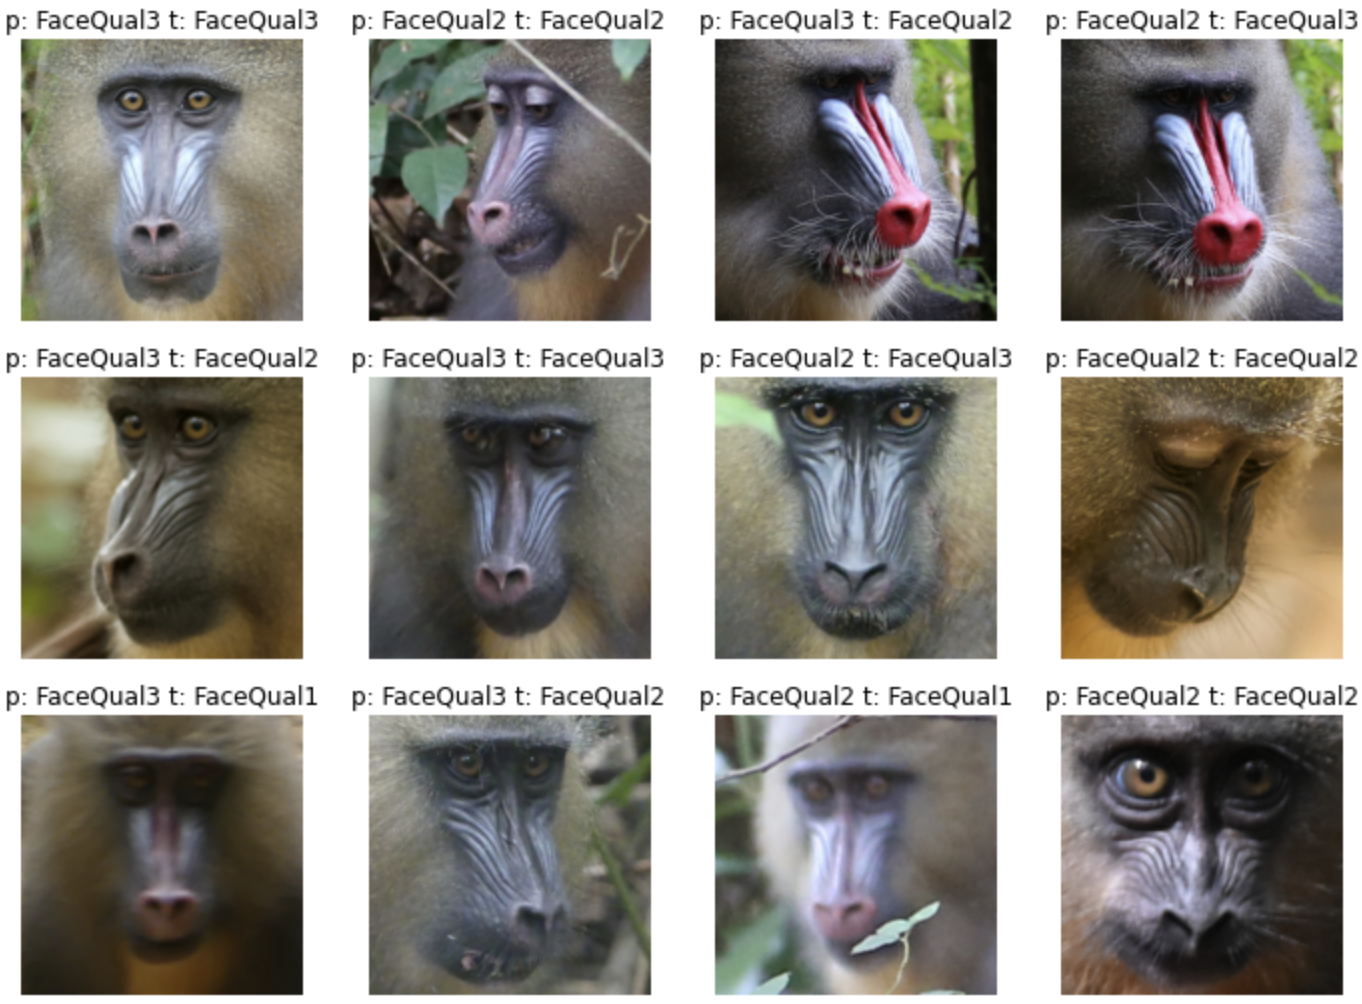
\includegraphics[width=200pt]{imgs/qualité/cr1/prediction1.png}
\end{center}

Mais les résultats sont trompeurs, en effet, le jeu de données est très déséquilibré, avec 10000 images de qualité FaceQual2 et 6000 de qualité FaceQual3 contre 250 et 1000 de qualité FaceQual0 et FaceQual1. Le modèle pourrait donc prédire tout le temps FaceQual2 et avoir 57\% d'accuracy par défaut.\\

Il faut donc gérer ce déséquilibre, et deux approches nous paraissent intéressantes :\\
\begin{itemize}
    \item dégrader des images de bonne qualité (downscale puis upscale et léger floutage) pour génerer des photos de mauvaises qualité (une mauvaise photo souvent a un manque de détails et/ou est flou).
    \item pondérer les classes de jeu de données pendant l'entrainement (accorder plus d'importance donc là où on aurait moins d'échantillons).
\end{itemize}

Voici un exemple de ce que pourrait être une dégradation d'images par rapport aux premières images :

\begin{center}
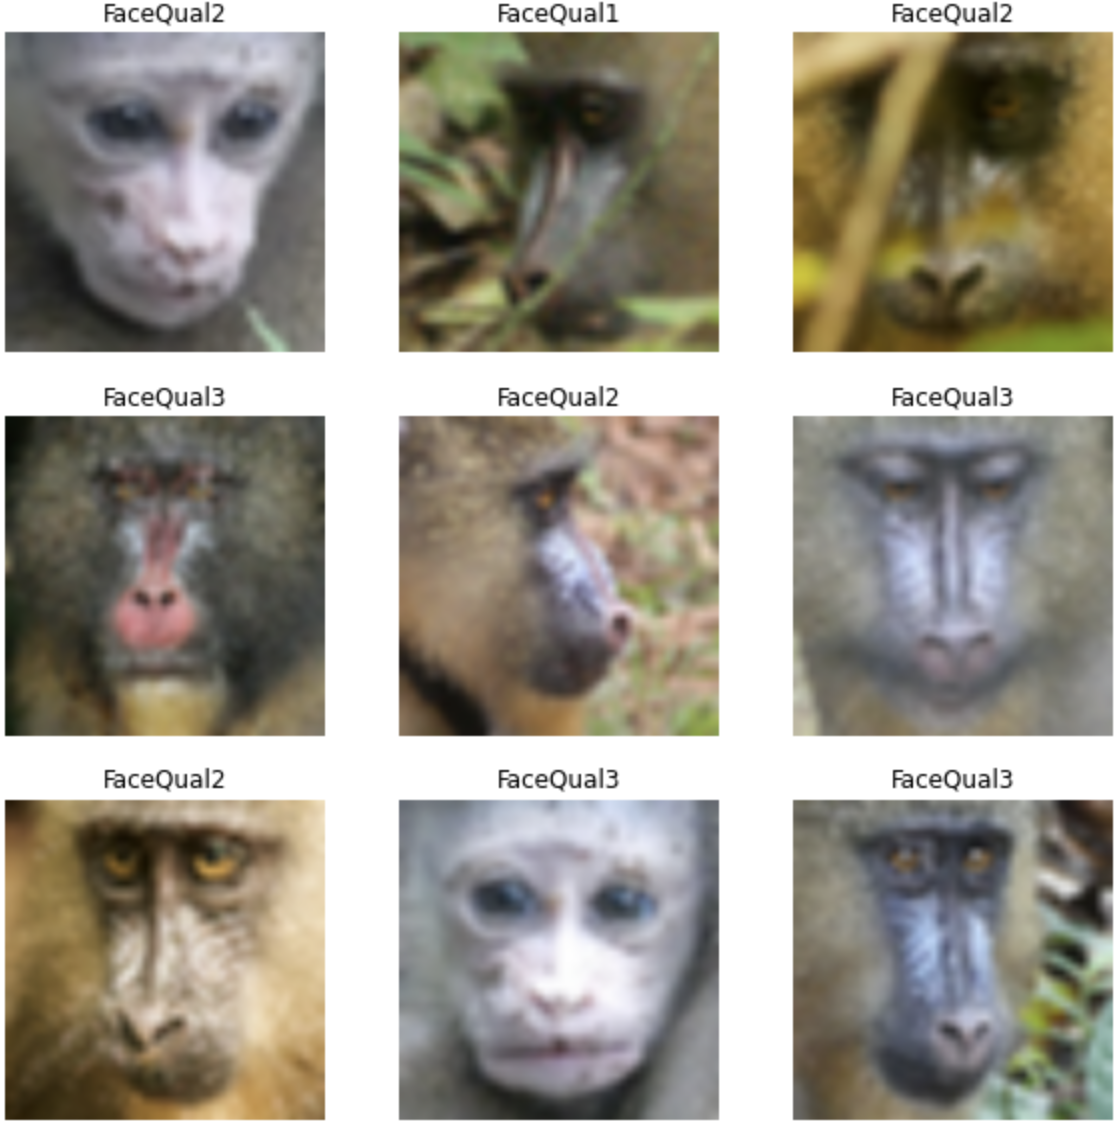
\includegraphics[width=200pt]{imgs/qualité/cr1/augmentation1.png}
\end{center}

Évidemment on peut faire varier le niveau de floutage et de dégradation de détails. On pourrait également imaginer appliquer un fort taux de compression JPEG ou augmenter le bruit artificiellement pour obtenir des images de basse qualité réalistes (tout cela étant des facteurs de basse qualité).\\

Ensuite, j'ai travaillé sur la matrice de confusion et le graphe ROC et commencer à comparer de manière plus complète les modèles.\\

Nous démarrons avec un transfer learning par VGG16/ImageNet suivi de deux couches complètements connectés, par enfin une couche softmax (probabilités).

Nous obtenons sur 10 epochs un rappel à 0.8 pour les 2 classes les plus représentés (FaceQual2/3) et 0.65 pour les autres (FaceQual0/1). Cela veut donc dire qu'une proportion correcte initiale d'échantillons est correctement classé.

\begin{center}
    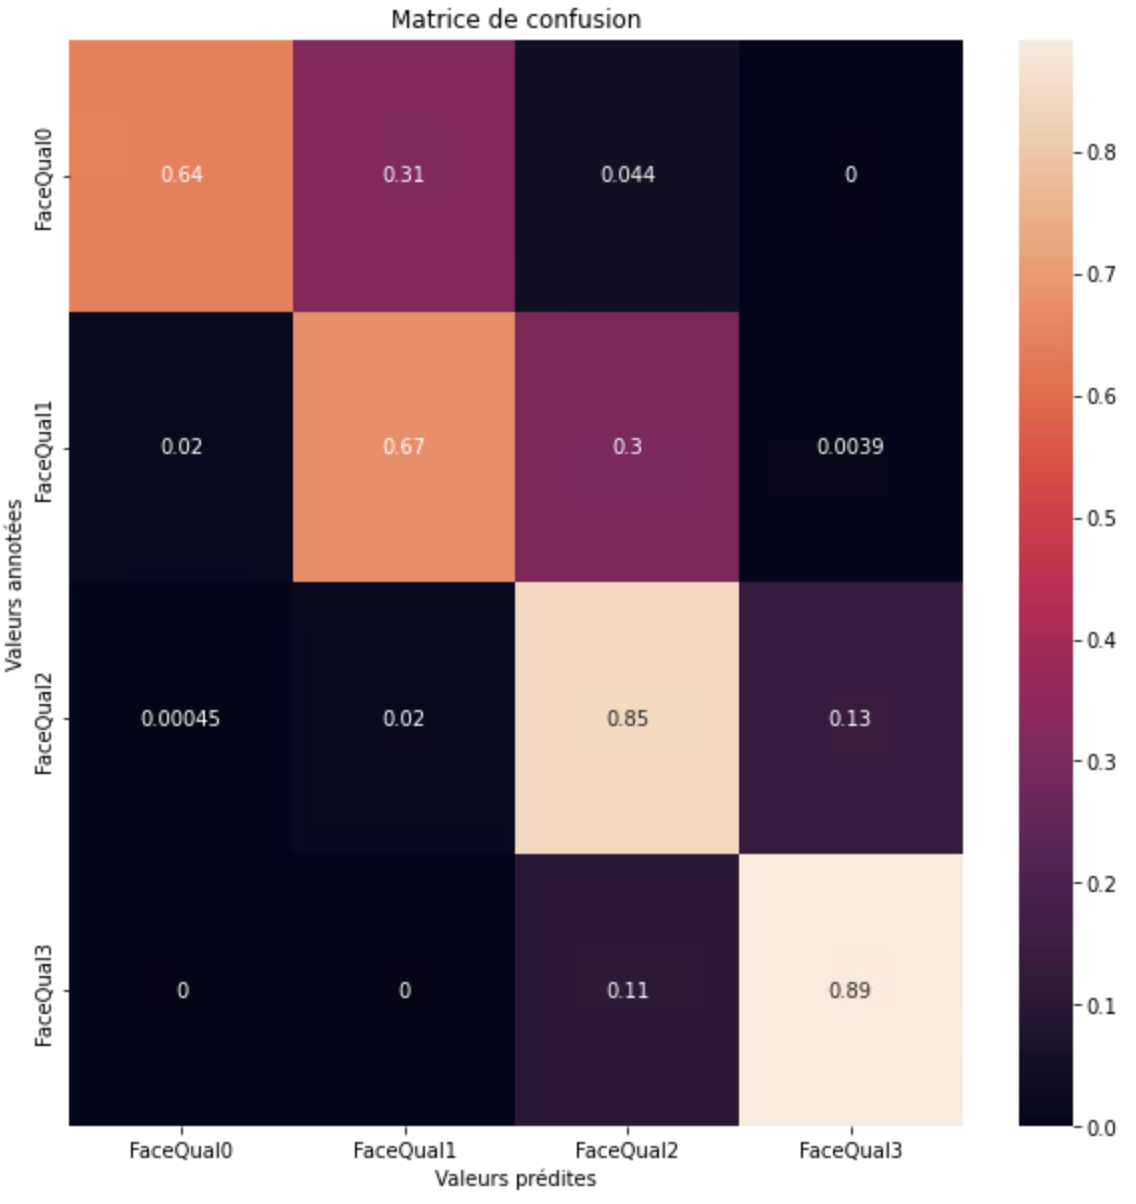
\includegraphics[width=170pt]{imgs/qualité/cr2/vgg16_000_confusion.png}
    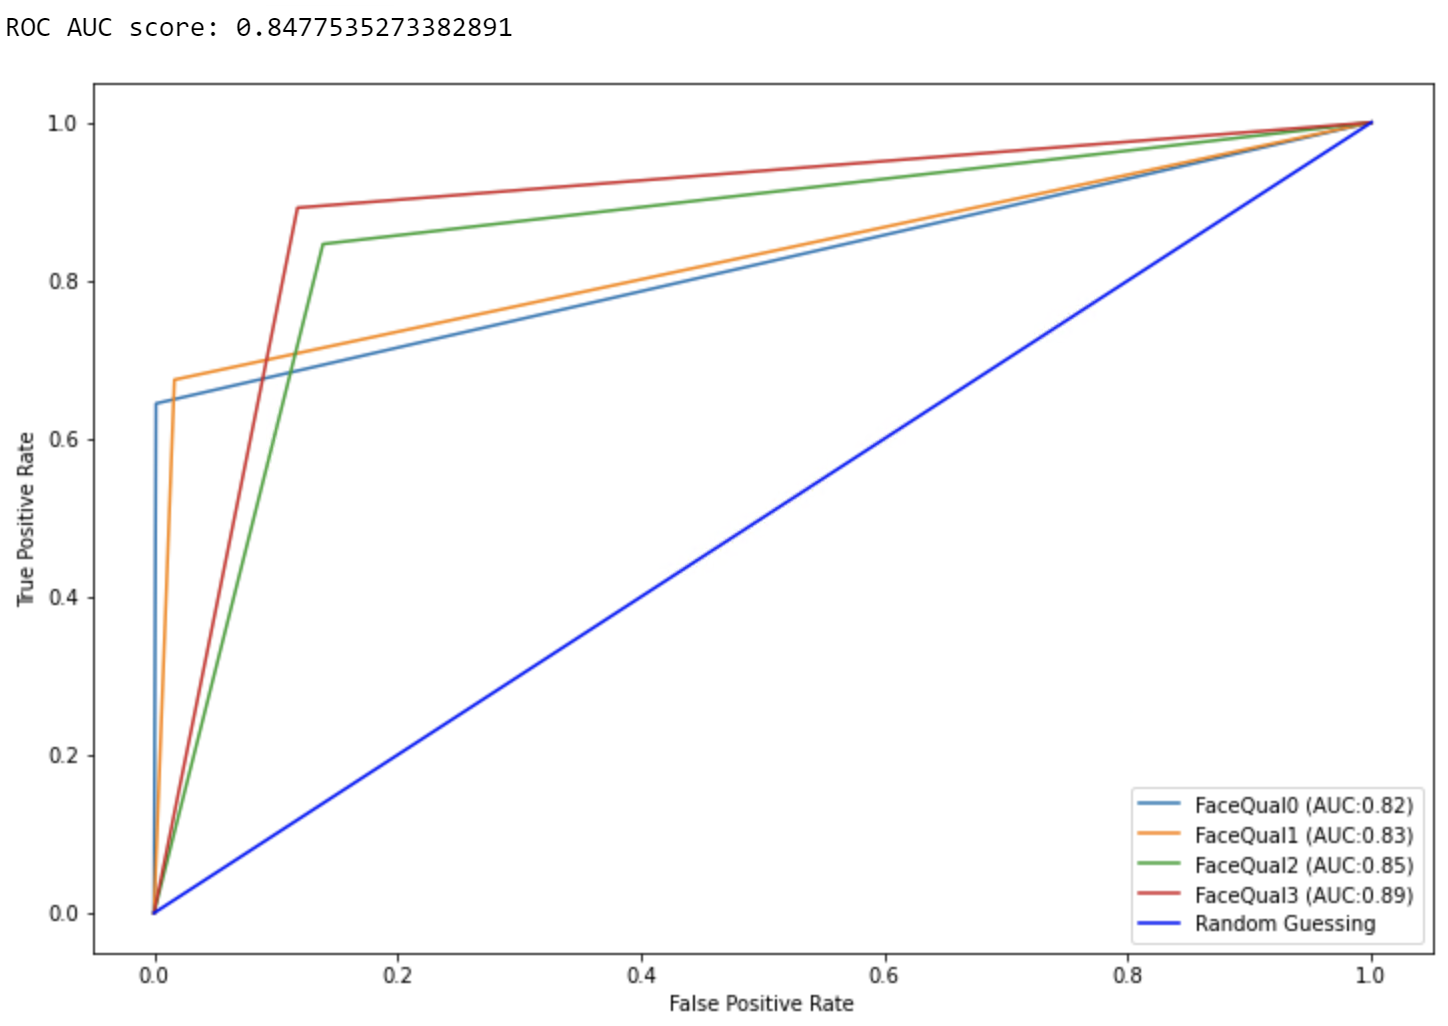
\includegraphics[width=170pt]{imgs/qualité/cr2/vgg16_000_roc.png}
\end{center}

Pour améliorer la situation, problématique sûrement à cause du déséquilibre des données, nous pouvons essayer d'abord la pondération des classes. Cela permet en effet d'améliorer largement le résultat de la classe la plus sous représentée (FaceQual0), avec un poids d'importance de 17. Seulement, une partie de l'apprentissage est troublée, d'une part car la classe FaceQual1 est partiellement confondue par la classe FaceQual0 et également du fait que beaucoup d'échantillons FaceQual2 sont classés en FaceQual0 (5\% des FaceQual2, représentant une bonne partie sachant que FaceQual2 possède énormément plus d'images).


\begin{center}
    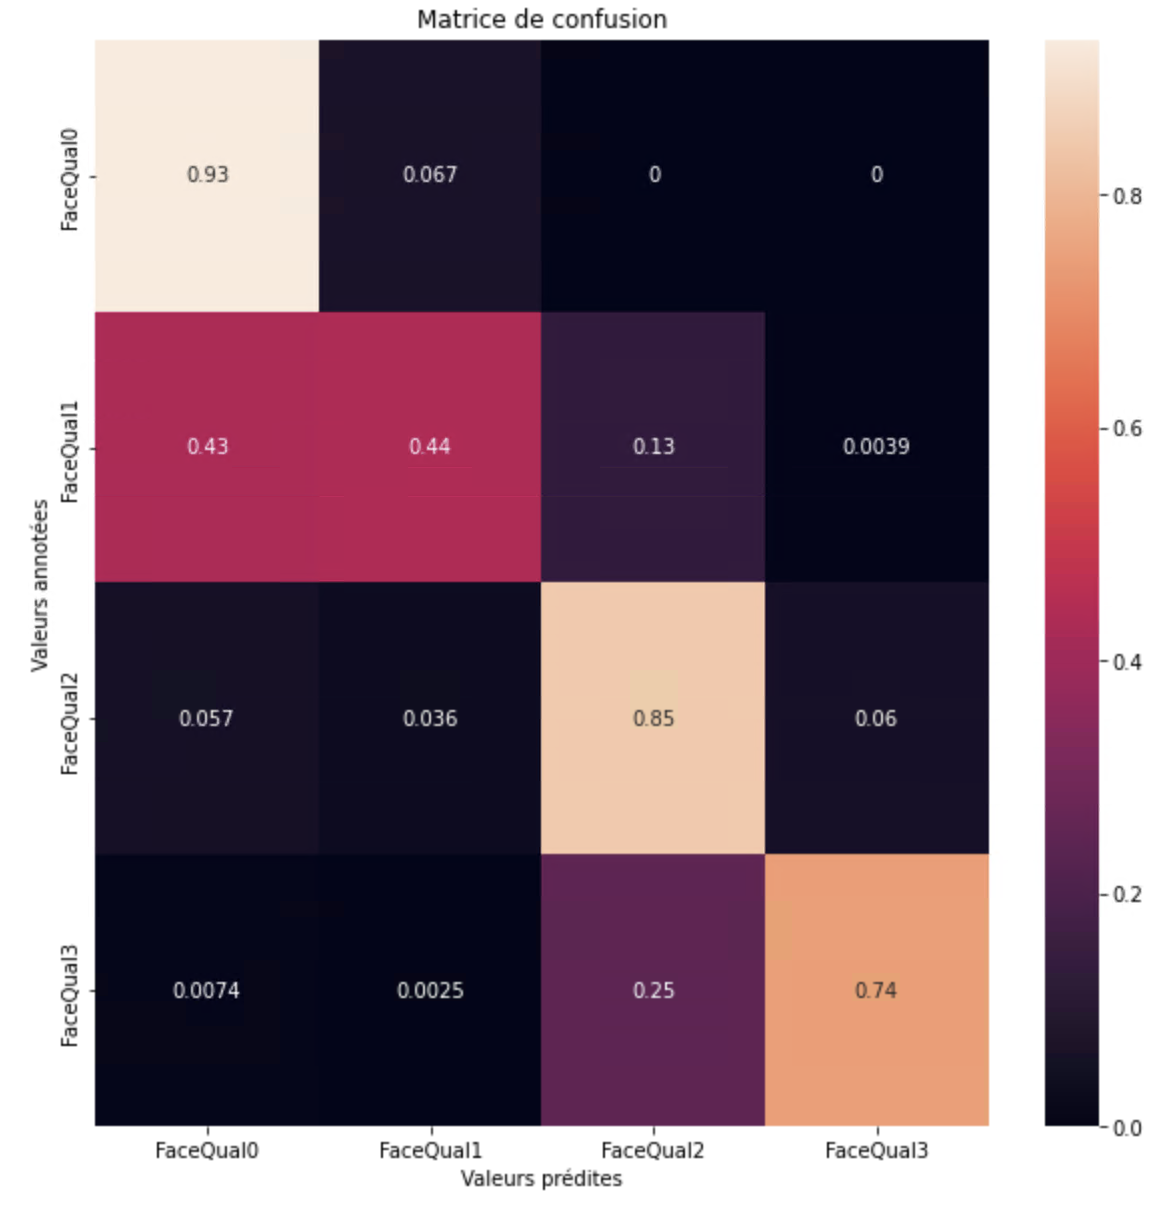
\includegraphics[width=170pt]{imgs/qualité/cr2/vgg16_010_confusion.png}
    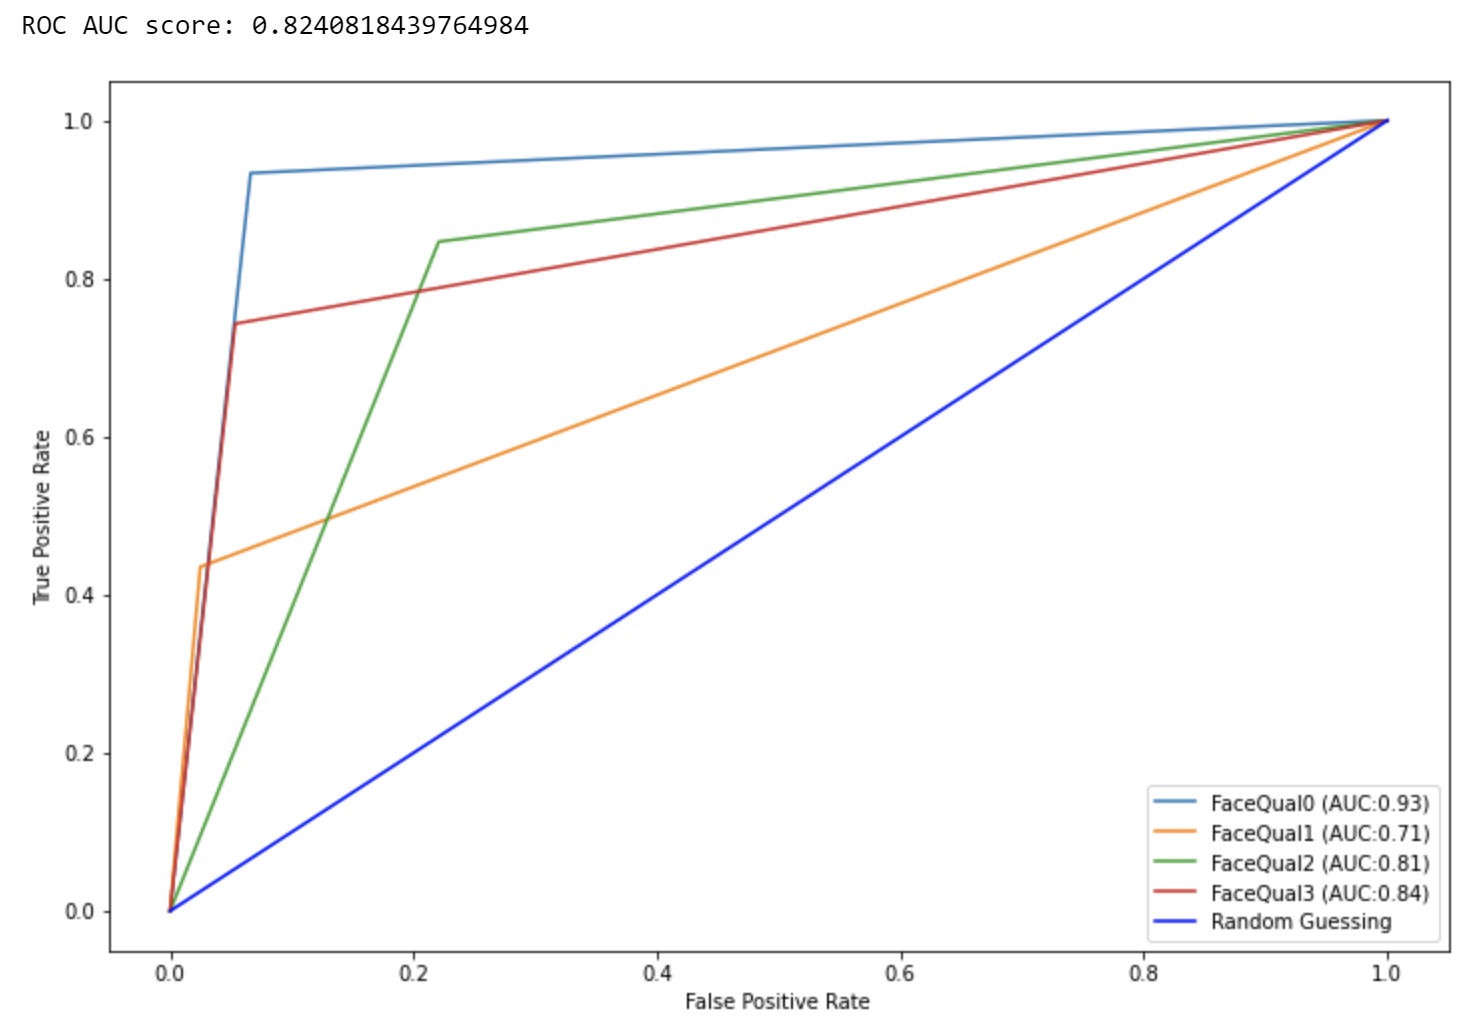
\includegraphics[width=170pt]{imgs/qualité/cr2/vgg16_010_roc.png}
\end{center}

Une piste est alors d'opérer un oversampling a priori sur la classe FaceQual0 pour avoir des poids de classes plus adéquats (moins grands). \\

Une fois testé, nous trouvons un rappel supérieur à la situation initiale sans cette fois-ci occasionner de dommages collatéraux. Le poids de la classe FaceQual0 après l'oversampling par copie/dégradation des images FaceQual3 est autour de 4, soit 4 fois moins qu'avant oversampling.

\begin{center}
    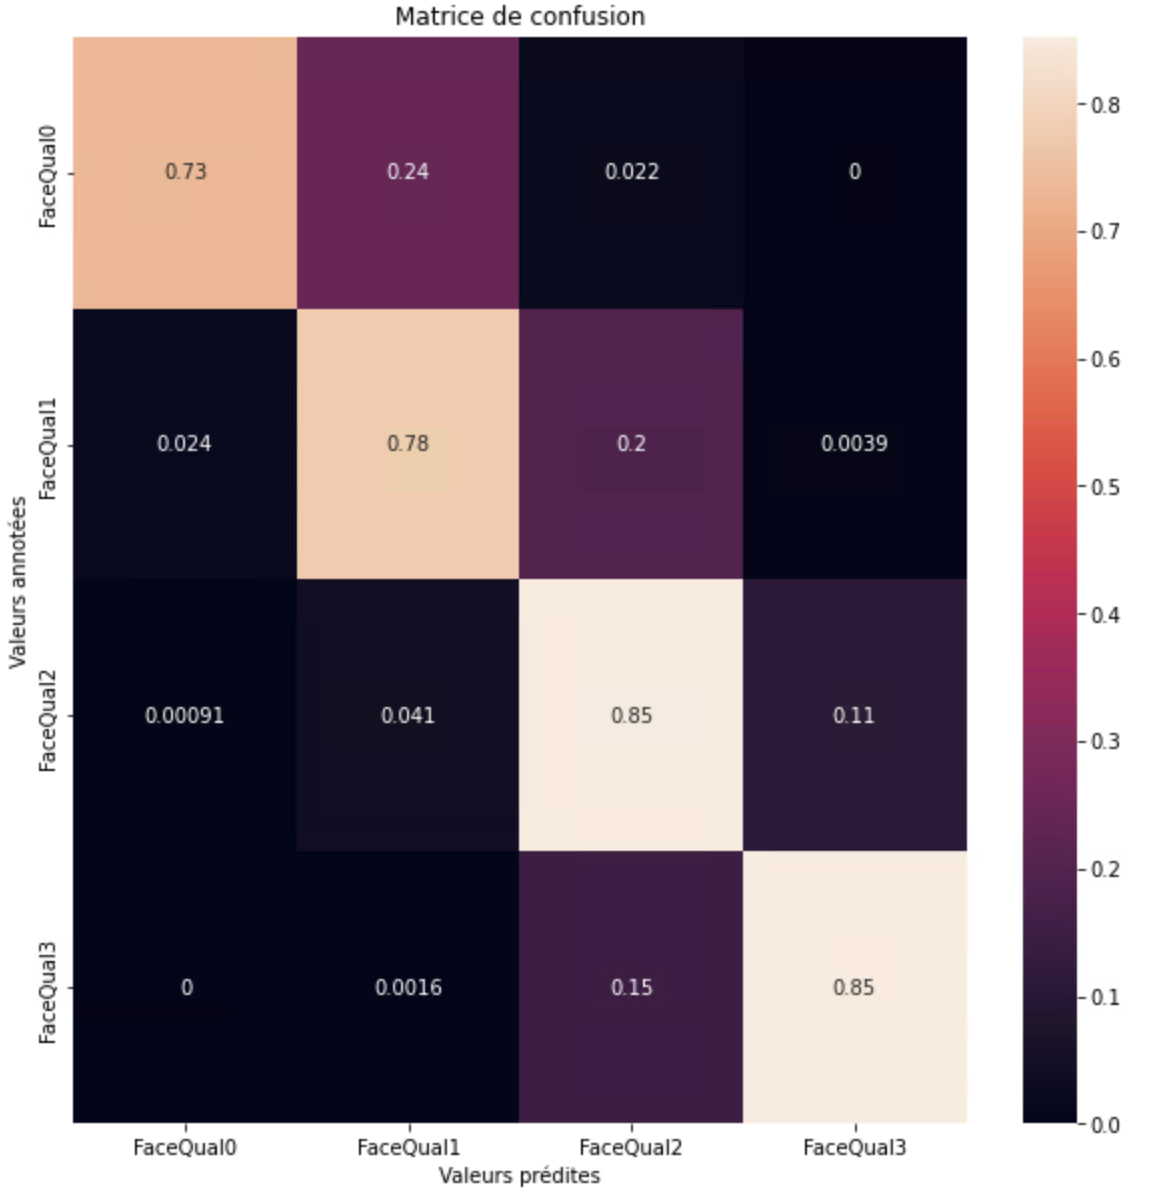
\includegraphics[width=170pt]{imgs/qualité/cr2/vgg16_011_confusion.png}
    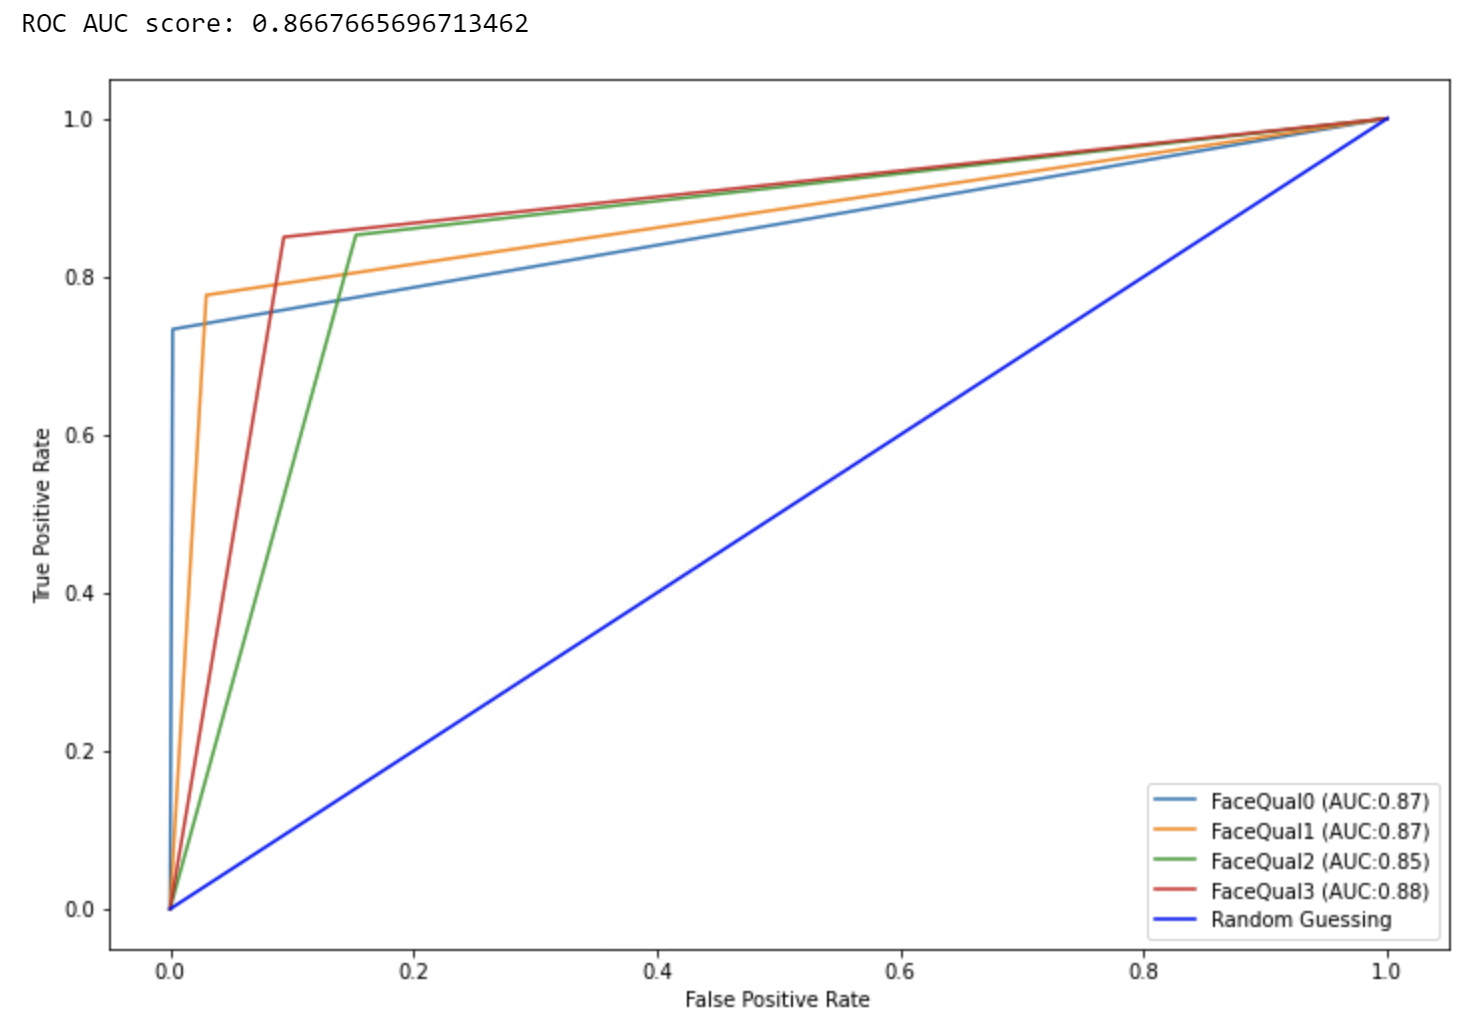
\includegraphics[width=170pt]{imgs/qualité/cr2/vgg16_011_roc.png}
\end{center}

\subsection{Base de données des métadonnées}
Avant le commencement du stage, les métadonnées étaient répartis sur plusieurs fichiers CSV. Cela induisait donc une certaine dureté pour y appliquer des modifications, ainsi qu'une rigidité pour utiliser les fichiers.\\

Alors nous nous sommes poser la question s'il pourrait être intéressant de créer une base de données pour organiser mieux le lien entre les métadonnées d'une image originale, d'une image portrait, d'un individu mandrill, etc...
Pour moi, le choix le plus cohérent était de partir sur une base de données SQLite, dite "file-based" (basé seulement sur le fichier). Ainsi, cela reste relativement simple à utiliser pour un centre de recherche non spécialisé en informatique puisqu'il n'y a pas de serveur, où tout le monde n'aurait pas envie de gérer ce dernier. Ce n'est pas non plus nécessaire car il n'y a pas réellement d'accès concurrent à cette base de données : elle sert avant tout pour les modèles d'entraînement ensuite.

\begin{center}
    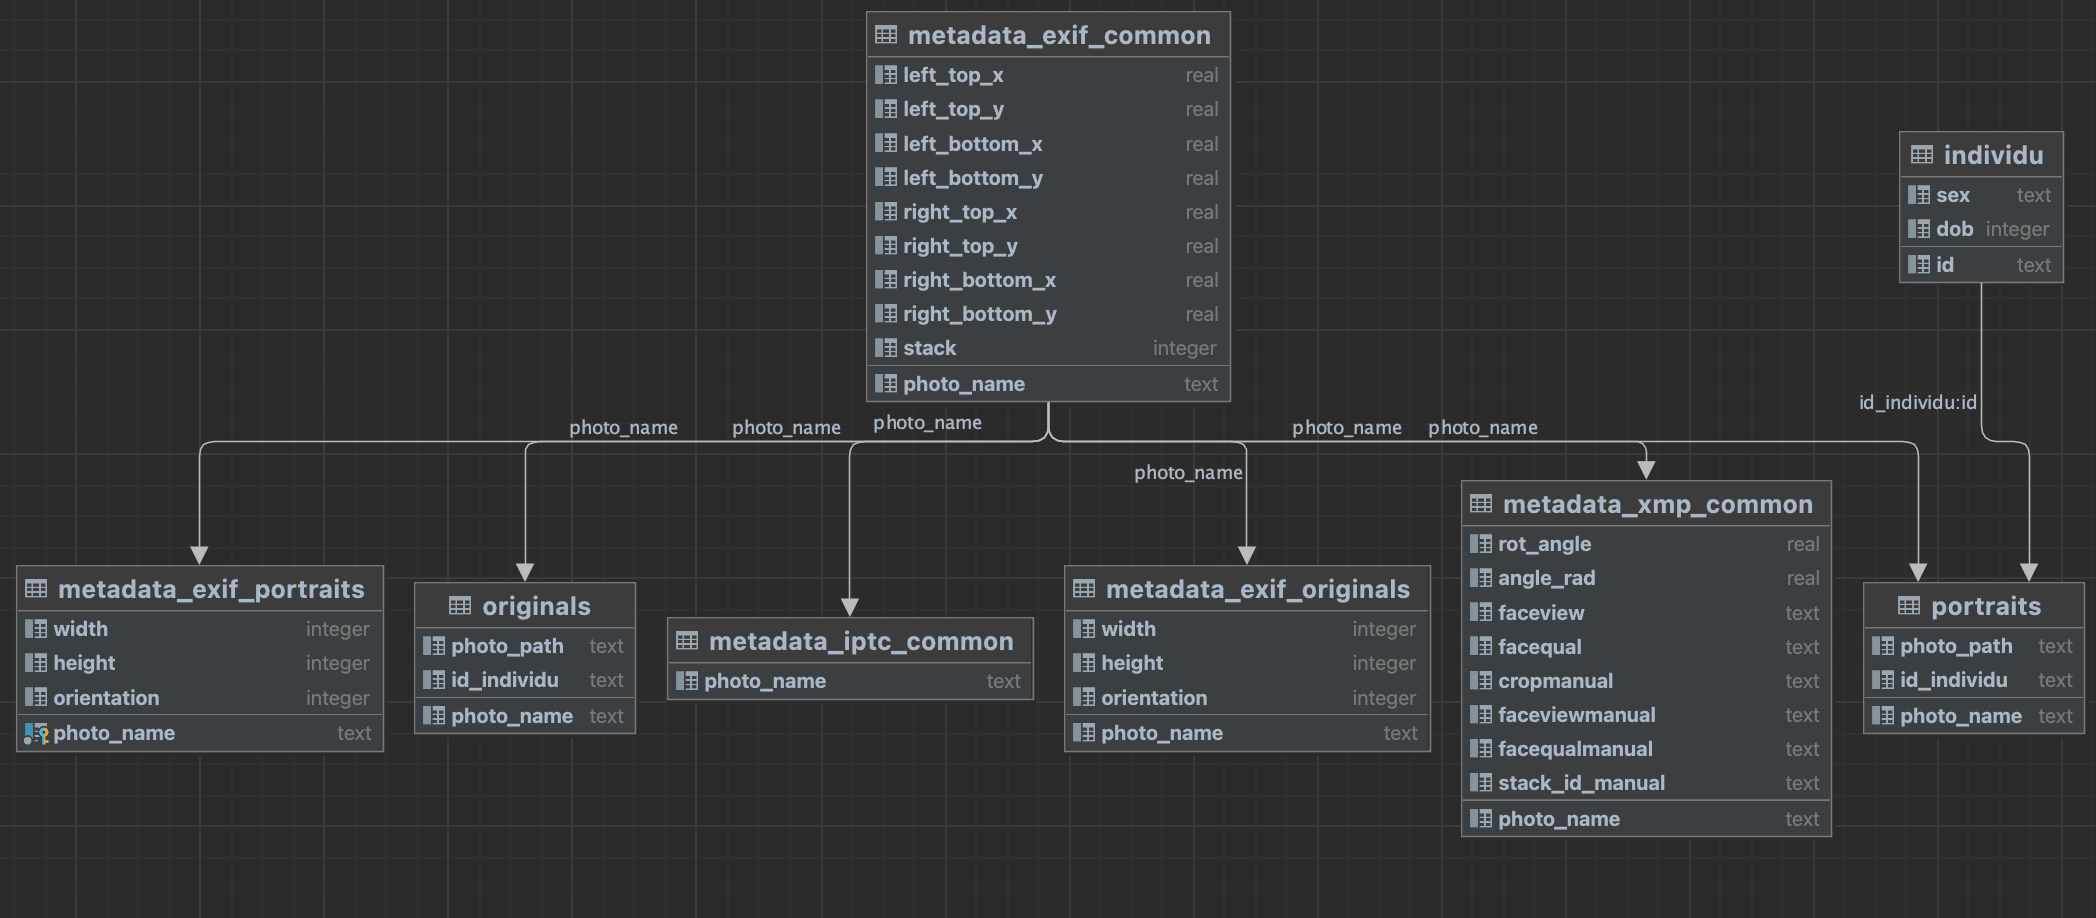
\includegraphics[width=345pt]{imgs/qualité/cr8/sqlite_schema.png}
\end{center}

\subsection{Docker}
Pour améliorer la portabilité de tous les scripts, j'ai mis en place Docker ainsi que Docker Compose. Docker est un logiciel qui permet de lancer un script avec son environnement "figé" de sorte qu'il fonctionne partout.\\

Voici donc des exemples de mes Dockerfile et docker-compose.yml : \\

Dans Dockerfile, nous précisions l'image de base (un OS ou, ici, un OS et une version de Python). Ensuite nous construisons l'image, en copiant les scripts locaux et installants les dépendances enregistrés dans un fichier requirements.txt (standard pour python pip). Enfin la commande ENTRYPOINT indique le point de départ de l'application, et CMD les paramètres par défaut, qui sont eux pour leur part surchargeables.
\begin{center}
    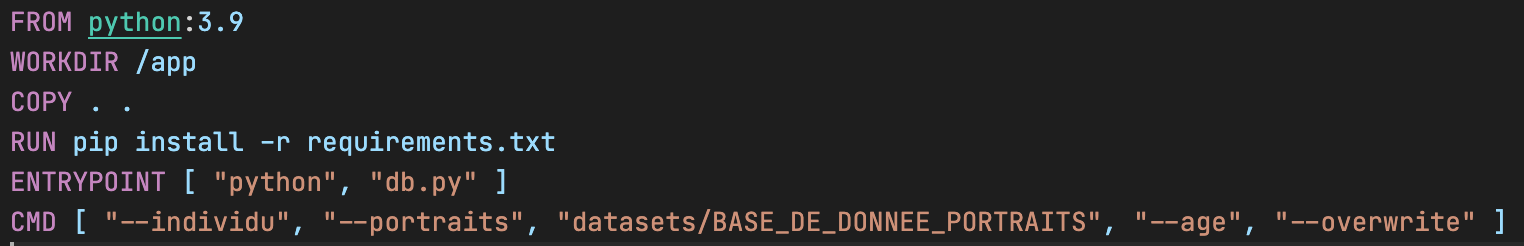
\includegraphics[width=345pt]{imgs/qualité/cr9/dockerfile.png}
\end{center}

Dans docker-compose.yml, nous pouvons composer des Dockerfile pour qu'ils soient dépendants les uns des autres ou simplement les lancer indépendamment des autres. Cela permet aussi de décrire les volumes / bind mounts directement dans un fichier de configuration (sans ces derniers les données seraient non persistantes).
\begin{center}
    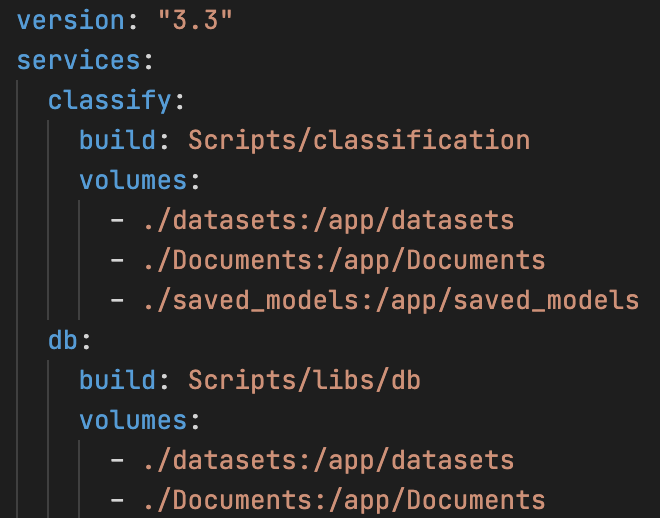
\includegraphics[width=345pt]{imgs/qualité/cr9/compose.png}
\end{center}

Voici un exemple de build des images et de run de l'image db. Comme le docker-compose indique l'utilisation de bind mounts, /app/Documents/Metadata/metadata.sqlite dans le container n'est autre que le fichier [projet]/Documents/Metadata/metadata.sqlite (persistant).
\begin{center}
    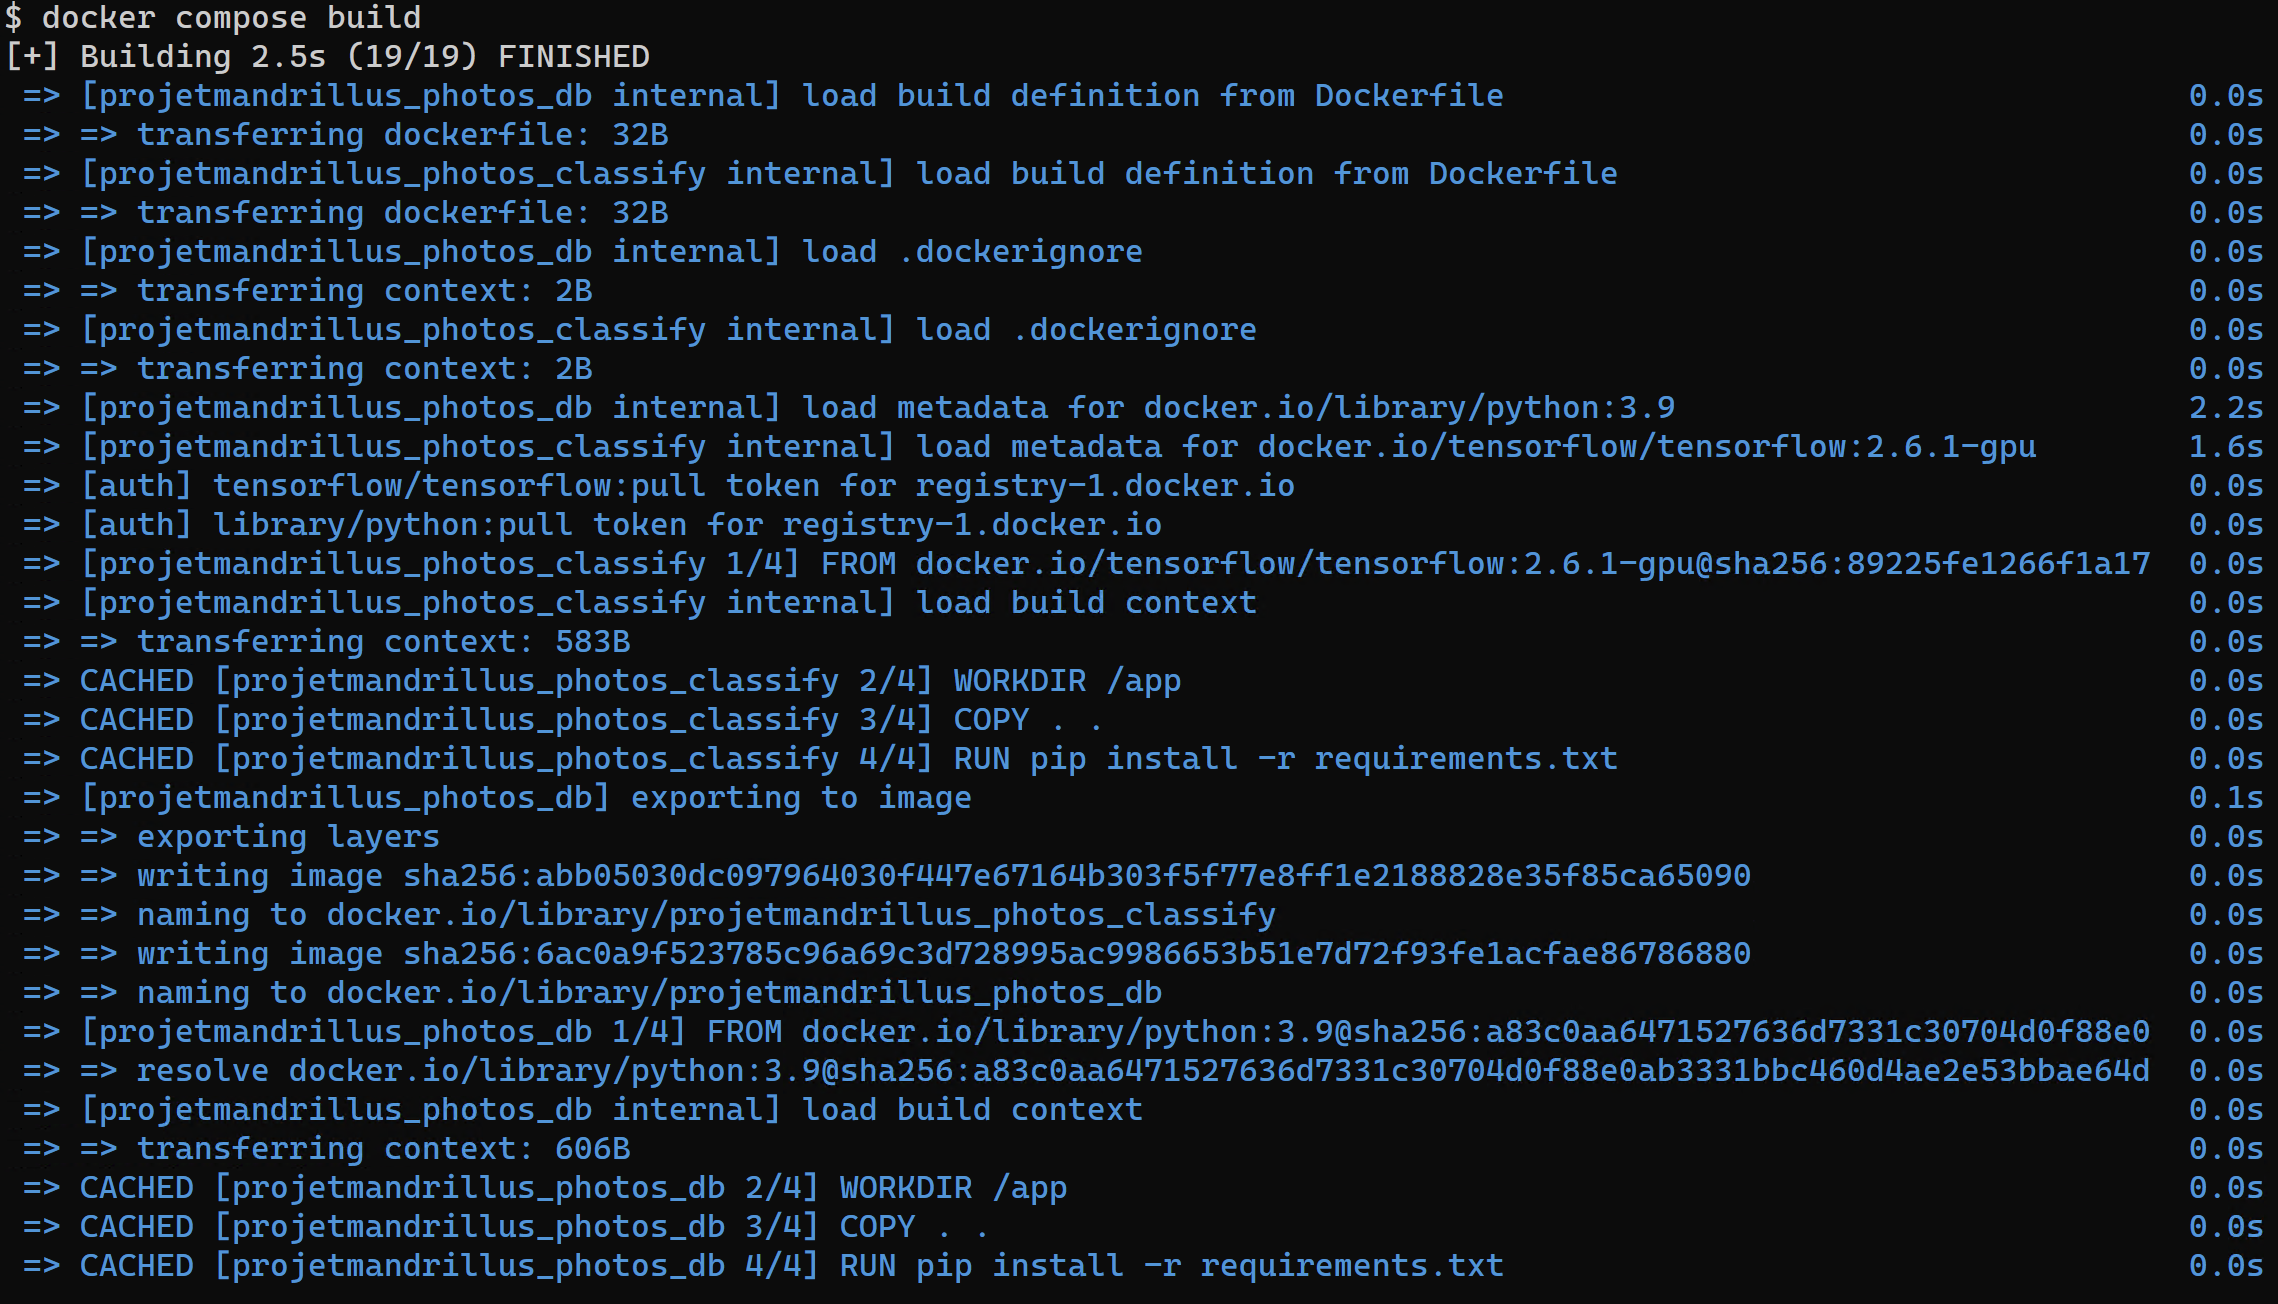
\includegraphics[width=345pt]{imgs/qualité/cr9/build.png}
    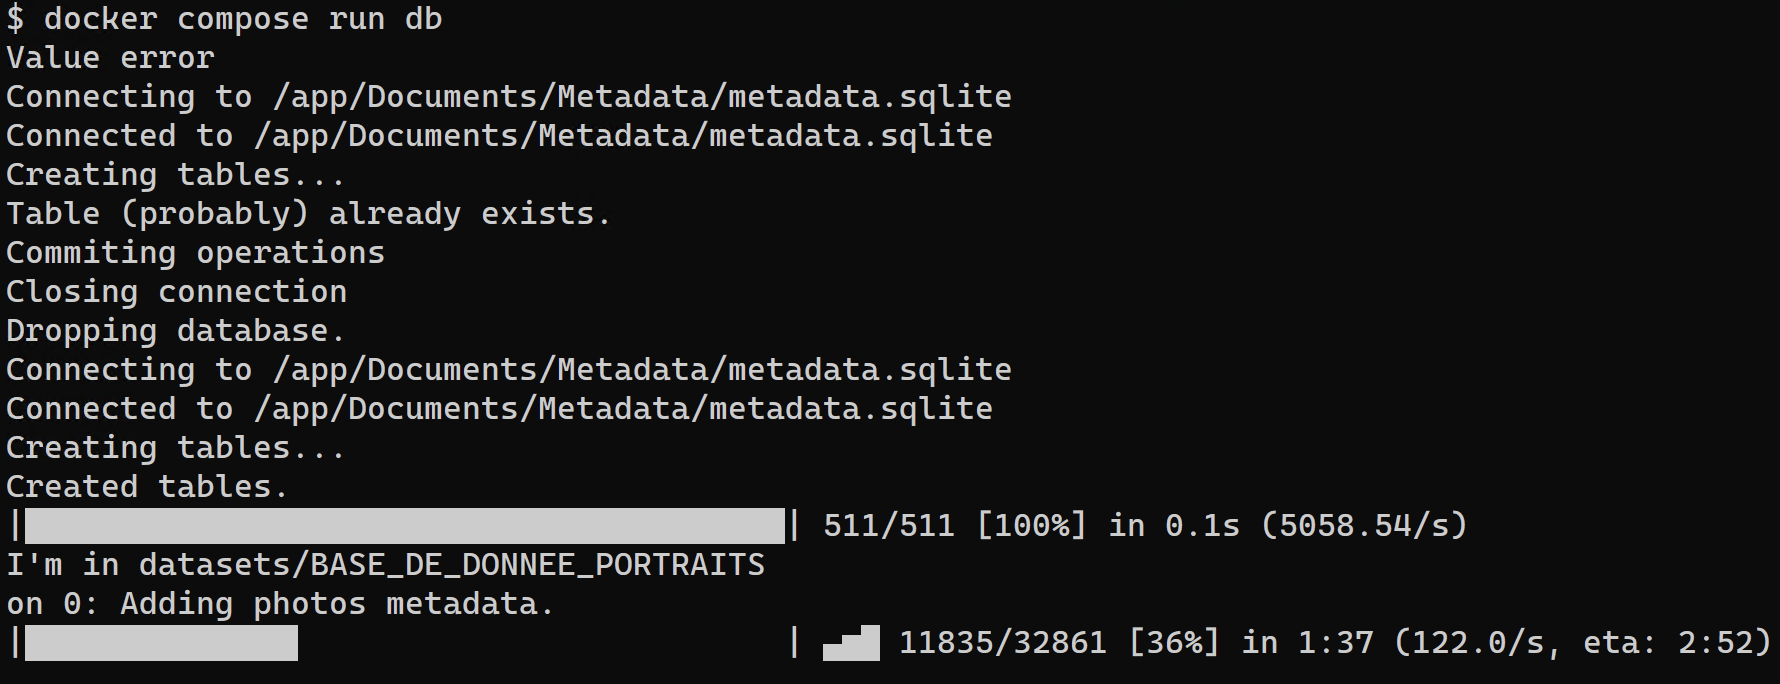
\includegraphics[width=345pt]{imgs/qualité/cr9/run.png}
\end{center}


\subsection{Tache 3}

\section{Conclusion} 

\section{Glossaire}
\clearpage
\printglossary[title={Glossaire}]

\section{Annexes} 

\section*{Remerciements}

Ce stage de master a été effectué dans le Laboratoire de Géopantouflisme de l’Institut de Physique du Globe de Paris, sous la direction de Napoléon Bonaparte, que je voudrais remercier pour la qualité du café qu’il sait faire. Émile Zola m’a aidé avec le logiciel LATEX de préparation de documents. Le logiciel de dessin utilisé appartient à l’Université de Cochabamba. Cette recherche a été menée à bien grâce à une bourse du Ministère des Anciens Ministres, et le microscope aquatique utilisé a été financé par le Centre National de la Recherche Parapsychologique.

https://stats.stackexchange.com/questions/181/how-to-choose-the-number-of-hidden-layers-and-nodes-in-a-feedforward-neural-netw

\end{document}
